\documentclass[aspectratio=169,11pt]{beamer}
\def\courseweek{4}
% Shared style for the Introduction to Information Geometry lecture slides.
% Compile the lecture .tex files from this directory.
\providecommand{\courseweek}{1}
\usepackage[T1]{fontenc}
\usepackage[utf8]{inputenc}
\usepackage[sc]{mathpazo}
\renewcommand{\sfdefault}{lmss}
\renewcommand{\ttdefault}{lmtt}
\usepackage{amsmath,amssymb,mathtools}
\usepackage{tikz}
\usetikzlibrary{arrows.meta,calc,positioning}
\usepackage{pgfplots}
\pgfplotsset{compat=1.18}
\usepackage{booktabs}

\definecolor{courseink}{HTML}{173749}
\definecolor{coursemuted}{HTML}{526674}
\definecolor{courseteal}{HTML}{0E7287}
\definecolor{coursecopper}{HTML}{B66B43}
\definecolor{courseline}{HTML}{D4E0E3}
\definecolor{coursepale}{HTML}{EFF5F5}

\setbeamercolor{normal text}{fg=courseink,bg=white}
\setbeamercolor{structure}{fg=courseteal}
\setbeamercolor{frametitle}{fg=courseink,bg=white}
\setbeamercolor{title}{fg=courseink}
\setbeamercolor{subtitle}{fg=coursemuted}
\setbeamercolor{block title}{fg=courseink,bg=white}
\setbeamercolor{block body}{fg=courseink,bg=white}
\setbeamercolor{alerted text}{fg=coursecopper}
\setbeamerfont{title}{family=\rmfamily,series=\bfseries,size=\fontsize{32}{37}}
\setbeamerfont{frametitle}{family=\rmfamily,series=\bfseries,size=\fontsize{26}{31}}
\setbeamerfont{normal text}{size=\fontsize{18}{22}}
\setbeamerfont{subtitle}{size=\fontsize{17}{21}}
\setbeamersize{text margin left=0.78cm,text margin right=0.78cm}
\setbeamertemplate{navigation symbols}{}
\setbeamertemplate{itemize items}[circle]
\setbeamertemplate{enumerate items}[default]
\setbeamertemplate{blocks}[default]
\setlength{\parskip}{0.22em}
\setbeamertemplate{footline}{%
  \leavevmode\hbox to \paperwidth{\hspace{.78cm}%
  {\color{coursemuted}\fontsize{8.5}{10}\selectfont Introduction to Information Geometry \hspace{.32cm} / \hspace{.32cm} Week \courseweek}%
  \hfill{\color{coursemuted}\fontsize{8.5}{10}\selectfont \insertframenumber\hspace{.17cm}/\hspace{.17cm}\inserttotalframenumber}\hspace{.78cm}}%
  \vskip.17cm
}
\setbeamertemplate{frametitle}{%
  \vspace{.13cm}
  \insertframetitle\par
  \vspace{.08cm}
}
\setbeamertemplate{title page}{%
  \vspace*{1.00cm}
  {\color{courseteal}\fontsize{10}{13}\selectfont\bfseries
  INTRODUCTION TO INFORMATION GEOMETRY\par}
  \vspace{.40cm}
  {\usebeamerfont{title}\usebeamercolor[fg]{title}\inserttitle\par}
  \vspace{.22cm}
  {\usebeamerfont{subtitle}\usebeamercolor[fg]{subtitle}\insertsubtitle\par}
  \vfill
  {\color{coursemuted}\fontsize{13}{16}\selectfont Christopher Lee\par}
  \vspace{.34cm}
}

\pgfplotsset{
  courseplot/.style={
    width=11.05cm,
    height=5.15cm,
    axis line style={coursemuted!75},
    tick style={coursemuted!65},
    ticklabel style={font=\scriptsize,color=coursemuted},
    label style={font=\normalsize,color=courseink},
    grid=major,
    major grid style={courseline!70,line width=.4pt},
    line width=1.45pt,
    legend style={font=\small,draw=none,fill=none,at={(.98,.03)},anchor=south east},
    clip=true
  }
}

\newcommand{\highlightmath}[1]{{\color{courseteal}#1}}
\newcommand{\thinrule}{\par\vspace{.25cm}{\color{courseline}\rule{\linewidth}{.8pt}}\par}

% A one-dimensional state space.  x=0 and x=1 are placed at 0 and 9 units.
\newcommand{\stateinterval}[1]{%
 \begin{tikzpicture}[x=1cm,y=1cm]
   \draw[courseink,line width=1.25pt] (0,0)--(9,0);
   \foreach \pos/\lab in {0/0,9/1} {
     \fill[courseink] (\pos,0) circle(2.7pt);
     \node[below=9pt,text=coursemuted] at (\pos,0) {\(\lab\)};
   }
   #1
 \end{tikzpicture}%
}

% Paired pages are separate frames in the PDF, with matching titles.
% Supply the whole frame body for each version; the instructor may edit them
% independently without changing overlay logic.
\newcommand{\coursepair}[3]{%
  \begin{frame}{#1}#2\end{frame}%
  \begin{frame}{#1}#3\end{frame}%
}

% Equilateral representation of the categorical simplex, in barycentric
% coordinates with vertices A=(0,0), B=(1,0), C=(1/2,sqrt(3)/2).
\newcommand{\coursesimplex}[1]{%
 \begin{tikzpicture}[scale=4.9]
  \fill[coursepale] (0,0)--(1,0)--(.5,.8660254)--cycle;
  \draw[courseink,line width=.65pt] (0,0)--(1,0)--(.5,.8660254)--cycle;
  \node[below left,font=\small] at (0,0) {A};
  \node[below right,font=\small] at (1,0) {B};
  \node[above,font=\small] at (.5,.8660254) {C};
  #1
 \end{tikzpicture}%
}

\title{Probability Laws, Means, and Variances}
\subtitle{Week 4 \(\cdot\) Lecture 1}
\date{}
\begin{document}
\begin{frame}[plain]\titlepage\end{frame}

\begin{frame}{A probability law is a mathematical state}
For three possible outcomes,
\[
\highlightmath{P=(p_A,p_B,p_C)},\qquad p_i\geq0,\quad\sum_i p_i=1.
\]
\vspace{.38cm}
The vector \((0.5,0.3,0.2)\) describes the probabilities
of all possible results of one observation.
\vspace{.45cm}
A single sample instead produces one outcome, such as B.
\end{frame}

\begin{frame}{Probabilities and numerical outcomes}
Let \(Z\) take values \(0,1,3\) with probabilities \(\frac12,\frac13,\frac16\).
\vspace{.2cm}
\begin{center}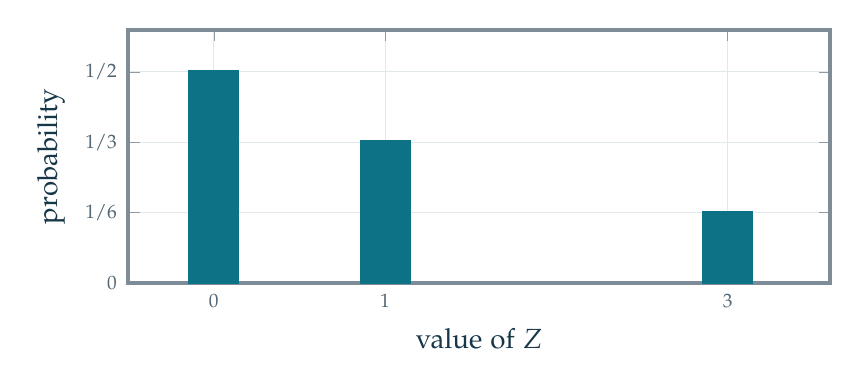
\begin{tikzpicture}
\begin{axis}[courseplot,width=10.5cm,height=4.8cm,
 xmin=-.5,xmax=3.6,ymin=0,ymax=.60,xtick={0,1,3},
 ytick={0,.1667,.3333,.5},yticklabels={0,$1/6$,$1/3$,$1/2$},
 xlabel={value of $Z$},ylabel={probability}]
\addplot[ybar,bar width=17pt,fill=courseteal,draw=courseteal]
coordinates{(0,.5)(1,.333333)(3,.166667)};
\end{axis}\end{tikzpicture}\end{center}
\end{frame}

\begin{frame}{Expected value as a function of probabilities}
For fixed numerical values \(z_i\), define
\[
\highlightmath{E_P[Z]=\sum_i z_ip_i}.
\]
\vspace{.55cm}
Changing \(P\) changes the expectation even if the possible values
of \(Z\) remain the same.
\vspace{.38cm}
This makes expectation a real-valued function on the simplex.
\end{frame}

\coursepair{The mean of a three-outcome law}{
For \(z=(0,1,3)\) and \(P=(\frac12,\frac13,\frac16)\),
\vspace{.45cm}
\[
E_P[Z]=0\cdot\frac12+1\cdot\frac13+3\cdot\frac16.
\]
\vspace{.48cm}
Find the expected value: \(\mu=\;?\).
}{
For \(z=(0,1,3)\) and \(P=(\frac12,\frac13,\frac16)\),
\vspace{.45cm}
\[
E_P[Z]=0\cdot\frac12+1\cdot\frac13+3\cdot\frac16.
\]
\vspace{.48cm}
The expected value is \(\highlightmath{\mu=\frac56}\).
}

\begin{frame}{Variance measures spread}
Write \(\mu=E_P[Z]\). The variance is
\[
\highlightmath{\operatorname{Var}_P(Z)=\sum_i p_i(z_i-\mu)^2}.
\]
\vspace{.48cm}
Equivalently,
\[
\operatorname{Var}_P(Z)=E_P[Z^2]-\mu^2.
\]
\vspace{.4cm}
It is another function on the space of distributions.
\end{frame}

\coursepair{The variance of the example}{
For \(z=(0,1,3)\), \(P=(\frac12,\frac13,\frac16)\),
and \(\mu=\frac56\), compute
\vspace{.36cm}
\[
E[Z^2]=0+\frac13+\frac96=\;?.
\]
\vspace{.30cm}
\[
\operatorname{Var}(Z)=E[Z^2]-\mu^2=\;?.
\]
}{
For \(z=(0,1,3)\), \(P=(\frac12,\frac13,\frac16)\),
and \(\mu=\frac56\),
\vspace{.36cm}
\[
E[Z^2]=0+\frac13+\frac96=\highlightmath{\frac{11}{6}}.
\]
\vspace{.30cm}
\[
\operatorname{Var}(Z)=\frac{11}{6}-\frac{25}{36}
=\highlightmath{\frac{41}{36}}.
\]
}

\begin{frame}{The Bernoulli family}
A Bernoulli random variable takes values \(0\) and \(1\).
\vspace{.42cm}
\[
\highlightmath{P_p=(1-p,p)},\qquad 0\leq p\leq1.
\]
\vspace{.38cm}
The parameter \(p\) determines the whole distribution:
\[
E[X]=p,\qquad \operatorname{Var}(X)=p(1-p).
\]
\end{frame}

\begin{frame}{Variance along the Bernoulli interval}
\vspace{-.18cm}
\begin{center}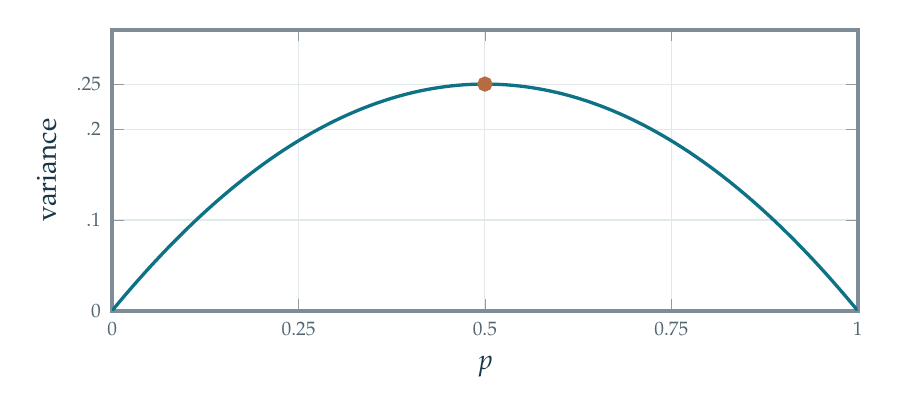
\begin{tikzpicture}
\begin{axis}[courseplot,xmin=0,xmax=1,ymin=0,ymax=.31,
 xlabel={$p$},ylabel={variance},xtick={0,.25,.5,.75,1},
 ytick={0,.1,.2,.25},yticklabels={0,.1,.2,.25}]
\addplot[courseteal,very thick,domain=0:1,samples=120]{x*(1-x)};
\addplot[only marks,coursecopper,mark=*,mark size=2pt] coordinates {(.5,.25)};
\end{axis}\end{tikzpicture}\end{center}
\vspace{-.1cm}
The variance is largest at \(p=\frac12\) and vanishes at the pure states.
\end{frame}

\begin{frame}{Expectation on the probability triangle}
Set \(P=(x,y,1-x-y)\) and \(z=(0,1,3)\).
\vspace{.4cm}
\[
\highlightmath{\mu(x,y)=0x+y+3(1-x-y)=3-3x-2y}.
\]
\vspace{.4cm}
\[
\frac{\partial\mu}{\partial x}=-3,
\qquad \frac{\partial\mu}{\partial y}=-2.
\]
\vspace{.38cm}
Probability laws supply an ordinary domain for multivariable calculus.
\end{frame}

\coursepair{Moving weight among outcomes}{
Let \(z=(0,1,3)\) and \(P=(\frac14,\frac12,\frac14)\).
\vspace{.38cm}
Compute the expectation:
\[
E_P[Z]=\;?.
\]
\vspace{.48cm}
Compare with the earlier distribution \((\frac12,\frac13,\frac16)\).
}{
Let \(z=(0,1,3)\) and \(P=(\frac14,\frac12,\frac14)\).
\vspace{.38cm}
The expectation is
\[
E_P[Z]=0\cdot\frac14+1\cdot\frac12+3\cdot\frac14
=\highlightmath{\frac54}.
\]
\vspace{.48cm}
It exceeds the earlier mean \(\frac56\): more probability lies on larger values.
}

\begin{frame}{A state and a sample answer different questions}
A probability distribution specifies the model's possible outcomes and
their chances.
\vspace{.43cm}
An observation records what occurred on one trial.
\vspace{.45cm}
An empirical distribution records the proportions of outcomes
in a collection of trials.
\vspace{.42cm}
These objects can all be drawn in the same simplex.
\end{frame}
\end{document}
